\documentclass[12pt]{article}
\usepackage[utf8]{inputenc}
\usepackage{graphicx}
\graphicspath{{images/}}
\usepackage{verbatim}

% Title Packages
\usepackage{titling}

% Timeline packages
\usepackage[TS1,T1]{fontenc}
\usepackage{array, booktabs}
\usepackage[x11names]{xcolor}
\usepackage{colortbl}
\usepackage{caption}

% Header packages
\usepackage{fancyhdr}
\pagestyle{fancy}
\setlength\headheight{26pt}


% Timeline custom command
\newcommand{\foo}{\color{LightSteelBlue3}\makebox[0pt]{\textbullet}\hskip-0.5pt\vrule width 1pt\hspace{\labelsep}}

% Fancy Header
\rhead{
\includegraphics[width=1cm]{swapblocks_icon.jpg}}

% Title Stuff
\setlength{\droptitle}{-10em} 
\pretitle{%
  \begin{center}
  \LARGE
  
\includegraphics[width=6cm,height=6cm]{swapblocks_icon.jpg}\\[\bigskipamount]
}


\title{SWAPBlocks\\}
%\title{SWAPBlocks \\A Cost Saving Blockchain Protocol\\
%For Asset Issuance \& Exchange}
\posttitle{A Cost Saving Blockchain Protocol\\
For Asset Issuance \& Exchange}

	  
\author{Lance Rogers \& Brandon McPherson}

\date{\today}

\begin{document}

\maketitle

\begin{abstract}
	

	
	
The rise of DAPP platforms over the last few years has sparked a movement to 
completely decentralize computing resources.  This movement has led to 
the creation of many irrational ecosystems where the cost and reliability of
applications is determined by the market price of the ecosystem's coin. % The unpredictable cost of running
%DAPPs today hinders many use cases from being implemented. 
While these ecosystems may work for simple contract execution,
many organizations that could benefit from the publicly verifiable nature of the
ecosystem, especially those subject to complying with changing regulation,
	are hesitant to do so due to uncertain cost. 
In order for mainstream adoption organizations must have the ability to manage
the cost of their own services.

In this paper, we discuss a new distributed ledger transaction verification
protocol designed to enable asset managers to control the cost associated with
transaction verification, data storage and transmission of their managed assets on 
	a public ledger.
This protocol allows for centralized, semi-centralized 
and decentralized control of assets registered on the ledger. 


\end{abstract}

\pagebreak

\tableofcontents

\pagebreak

\section{Introduction}



The SWAPBlocks protocol is a complement to distributed ledger technology that enables
asset managing entities to register and control the transfer of assets on a distributed
ledger.  The SWAPBlocks network is an implementation of this protocol aimed at creating a network
of clearinghouses, making automated swap transactions between all asset classes possible.  Such a network
would remove many of the cost associated with hiring expert facilitators, provide a publicly verifiable
lineage of each asset, and eliminate the need for two parties to convert to a common currency.


SWAPBlocks node API’s will enable seamless integration into 
existing record keeping infrastructure and encourage fast adoption. These 
features enable regulated and physical assets to be exchanged as quickly, cheaply
and easily as cryptocurrency.

The amount of data needed for rights transfer can vary based on the asset class
jurisdiction and the asset issuer.
For this reason data used for additional verification is hashed and discarded by the
main network, passing on the responsibility of maintaining data details to
the asset issuer. 
This helps prevent the chain from becoming bloated with information irrelevant 
to the majority of the network.  By checking the hash on the network against 
the hash of the data provided by the registering entity counterparties can easily 
confirm data integrity and detect tampering by the asset manager.


\section{SWAPBlocks Protocol}
\subsection{Base Protocol}
Assets are registered on the network by creating a new asset object containing 
a unique\_id, a pointer to the issuer, an asset\_id created by hashing the pointer 
and unique\_id, a prepended weight associated with the number of signatures needed 
for transactions to be considered valid and a valid\_through\_date.  Once the asset 
is created it is signed by the issuer and broadcast to the network as an asset 
genesis transaction. The issuer then runs a node supporting the network and listening 
for transactions containing its managed assets.

When a transaction is detected containing a managed asset the issuer processes the 
transaction and decides to approve or reject it.  This approval can be 
determined by any preset or future case set by the issuer.  Some examples include 
verifying that the address receiving the asset is legally allowed to receive the asset, 
verifying that an appropriate transaction fee has been included in the transaction, 
verifying that an encrypted form sent with the transaction contains the correct 
information, etc….  It is the responsibility of the issuer to provide counterparties with 
asset transfer instructions and the responsibility of the consumer to interpret
the instructions.

To approve a transaction the issuer must sign the transaction and rebroadcast 
the transaction to the network. Once the transaction is signed by the issuer
the transaction will be eligible for the next block.  
If the issuer does not approve the transaction it will
time out and be cleared from all network nodes.

\subsection{Consortium Extension}

The base protocol forces all transactions pertaining to a specific asset through 
the issuer's node which can cause performance issues and creates a single point 
of failure.  To solve these problems, issuers can extend the base protocol by 
forming consortiums that operate under consortium agreements.  These consortium 
agreements keep track of member nodes, consortium governing rules and 
verification scripts.  By joining a consortium the issuer agrees to process 
transactions of member nodes in accordance to the agreement and/or store 
the additional data attached to member transactions.

\section{Consortium}

Leaving an entity to verify all transactions pertaining to its managed assets can create 
a centralized bottleneck.  To solve this problem a municipal node can join or create a consortium.  
Consortiums are groups of nodes that require the same transaction verification process.  
This can be the full transaction verification needed or a subset of the full transaction verification. 
Consortiums follow rules set out in a consortium agreement which includes a transaction 
verification script, consortium data packet storage and routing fees.

Consortiums create a semi-decentralized, semi-private transaction verification network that 
enables a central entity to benefit from the distributed properties of a decentralized network.  
Consortiums also reduce the amount of trust needed to interact with any particular central 
entity since the operating agreement can be read and verified on the blockchain.

\begin{figure}[h]
	\centering
	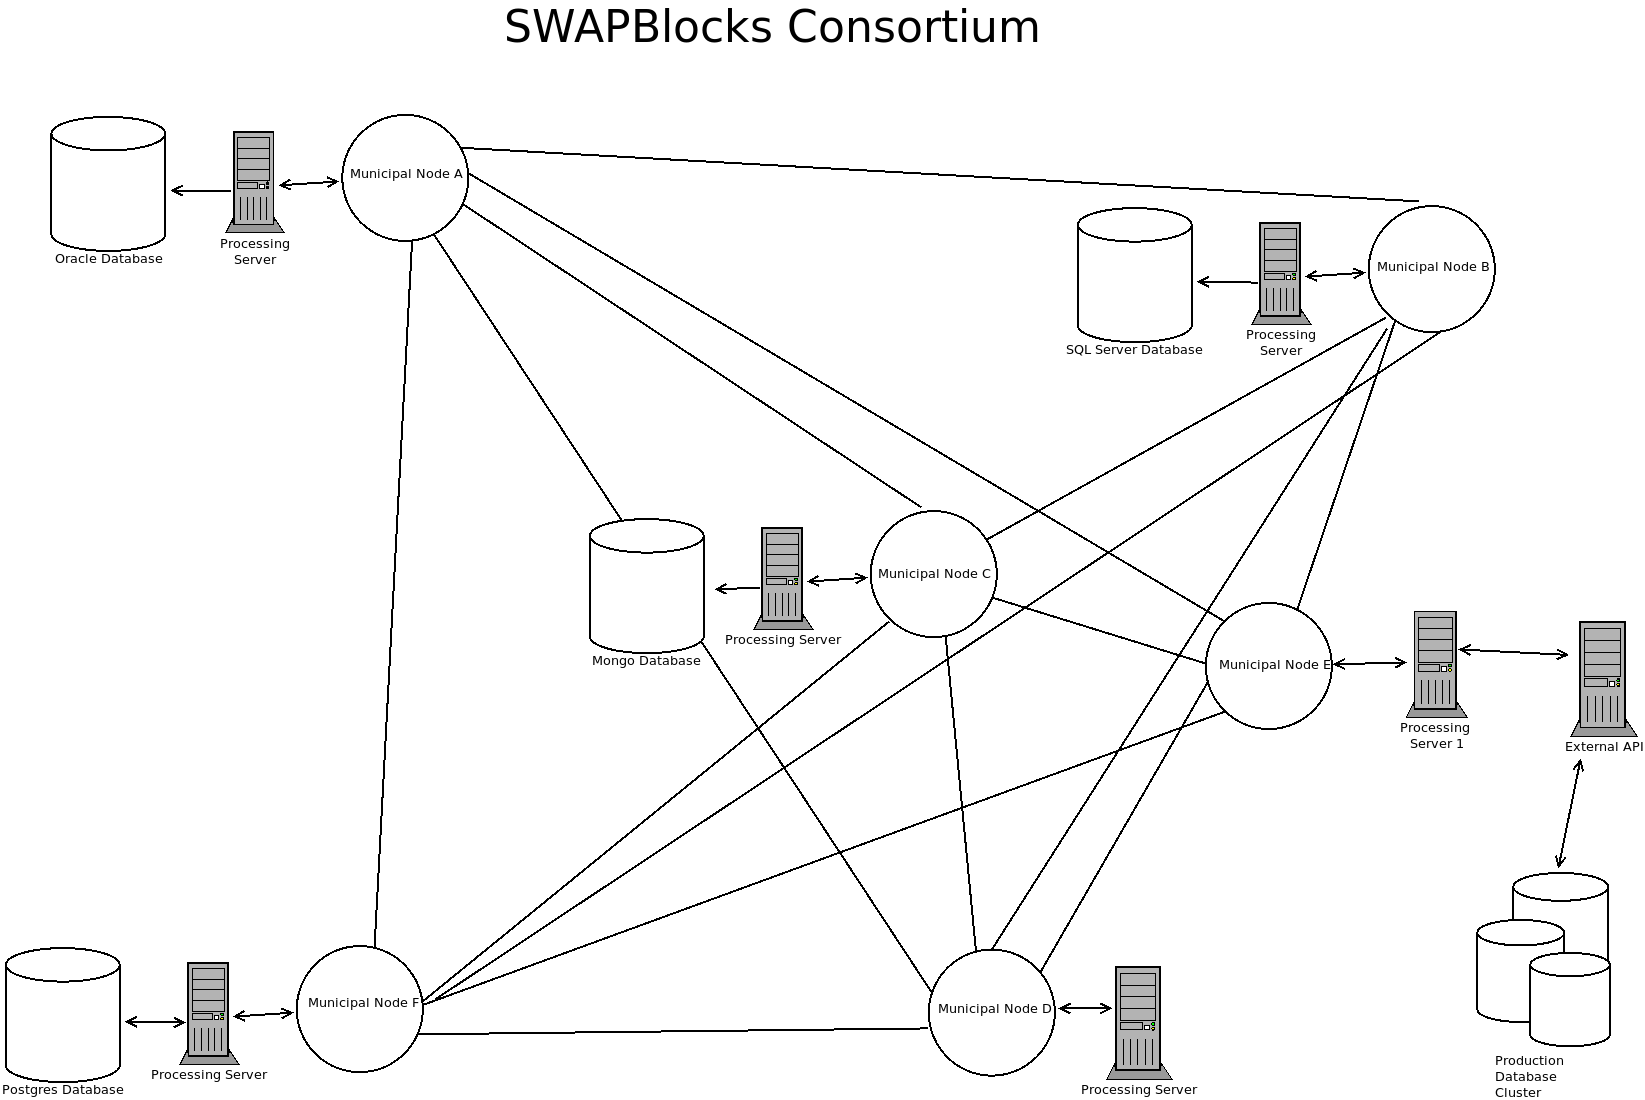
\includegraphics[width=.85\textwidth]{consortium}
	\caption{Consortium data storage infrastructure can vary between consortium nodes.} 
	\label{fig:consortium}
\end{figure}


\subsection{Consortium Agreement}

A consortium agreement is stored 
on the blockchain and acts as the operating agreement for all member nodes. 
This agreement outlines the processing script, consortium 
members, number of member signature needed for amendments, routing fee prices, a 
list of all member nodes' static IP’s, etc….

\subsection{Consortium Routing}


In order to limit the impact asset transactions have on the network as a whole mining 
nodes receive a portion of the attached fee for sending asset transactions to the correct
consortium network.  Consortiums can adjust the fee regularly to stay competitive for both
consumers and miners or build out a network. 
For a miner to 
increase their chances of receiving a routing fee they can store a dictionary 
of consortiums' node addresses for quick routing.



\subsection{Routing DAG}


The routing DAG contains the information associated with the routing of asset 
transfer transactions.  For example node X receives the transaction and performs standard 
verification, signs the transaction and broadcast it to the network where it is picked
by node Y. Node Y looks up the consortium's address in its dictionary of 
consortiums, signs and sends the transaction to consortium member node A. Node A performs 
consortium verification, signs the transaction and routes the transaction directly to 
municipal node F.  Node F verifies and signs the transaction. 
Now this transaction can be included in a block.  When the 
transaction is included in a block the last 3 addresses to sign the transaction 
receive shares of the attached routing fee.  Each signature in the routing DAG points 
to the previous one and can only contain one signature per level of verification.  
The first signature can be any node in the network, 
the second signature can be either a consortium member or the municipal node 
and the third can only be the municipal node.  The amount of signatures needed 
is determined by the asset's assigned weight value. 
%There will be a disincentive for altering the DAG.




\section{Node States}

SWAPBlocks assets view nodes in three different states. The state that the node is viewed in 
by the asset determines the level of verification the node is allowed to and should
perform.


\begin{enumerate}
	\item Standard Node State
		\begin{itemize}
			\item{Any network node that has no ownership stake in an asset}
			\item{Checks that each transaction output points to valid UTXOs
				and that all signatures are correct.}
		\end{itemize}
	\item Consortium Node State
		\begin{itemize}
			\item{Node belongs to the same consortium as the asset issuer,
				thus abiding by the same consortium agreement.}
			\item{Typically responsible with processing  or storing
				consortium data packets containing information 
				needed for additional verification}
		\end{itemize}
	\item Municipal Node State
		\begin{itemize}
			\item{Node owned by the asset issuer.}
			\item{Responsible for verifying municipal data packets.}
			\item{Responsible with updating their own outside record keeping systems with
				with status changes of registered assets.}	
		\end{itemize}
\end{enumerate}

\begin{figure}[h]
	\centering
	
\includegraphics[width=.85\textwidth]{node_space}
	\caption{Node space in relation to some registered asset}
	\label{fig:nodespace1}
\end{figure}


Figure \ref{fig:nodespace1} represents the node space in relation to a registered asset.
Each circle represents a node and each color represents the state that the
node is in for a particular asset.  The yellow circle represents the municipal node, meaning
that the yellow node registered and manages the asset.  The red circles represent consortium 
nodes, meaning that each red node is a member of the same consortium as the municipal node.
The black dots represent standard network nodes that do not have any special permission or
obligation to provide additional verification for this asset.  

%As you can see each node state inherits the traits of the previous state.





\section{Asset Registration}

Municipal nodes register assets in an asset genesis transaction.  When 
an asset is registered there are only 4 required fields, the registering node's 
pub key, the consortium's address if there is one, a UAI and a valid\_through date.  
This valid\_through date is the date that the entity guarantees the information 
about the asset to be correct.  The asset must be verified through an asset probe 
transaction to update the valid\_through date.

\subsection{Asset ID}

Assets on the SWAPBlocks network are represented by a unique asset ID (UAI).  
The UAI is created by hashing the consortium address with the municipal address 
and then hashing that with the municipal ID to create the base\_id.


% ASSET ID DIAGRAM HERE


% Add below to diagram somehow
% Asset Base ID:
% e3cc54301269c1c54afeb86e4391a9ad80d40484a9b0db0e6618b835decc9628

Now that the base ID has been formed the municipal node assigns 
a weight, determining the level of verification required to transfer 
the asset, and prepends the weight to the beginning of the asset ID.

\subsection{Weights}

Assets are assigned weights when they are first created. These weights are used to
to determine the level of verification a transaction containing the asset needs before
being eligible to be
included in the next block. Weight is calculated based on the number of valid signatures
a transaction has in it's routing DAG.


\begin{itemize}
	\item Weight 0, Standard Verification
		\begin{itemize}
			\item{Default verification requiring the trans-action to include
				valid UTXOs and signatures.}
		\end{itemize}
	\item Weight 1, Consortium Level Verification
		\begin{itemize}
			\item{Transactions must pass weight 1 verification and contain an
				additional signature from a consortium node.}
			\item{Assets with this weight may require a consortium data packet
				to be sent along with every transfer transaction}
		\end{itemize}
	\item Weight 2
		\begin{itemize}
			\item{Transactions must pass weight 0 verification and include a 
				municipal signature in the routing DAG.}
			\item{Consortium nodes can perform consortium verification on
				the consortium data packet, sign the DAG and send the
				transaction directly to the municipal node, enabling
				the consortium node to receive some of the routing fee.
				If this verification has been done and signed off by
				a trusted consortium node the municipal node does not
				need to reverify and will only need to
				perform municipal verification.}
		\end{itemize}
\end{itemize}

% ADD Weighted Asset Diagrams Here


\section{Transactions}

\subsection{Transaction Types}
There are 5 basic types of transactions in the SWAPBlocks ecosystem.

\begin{enumerate}
	\item Currency
		\begin{itemize}
			\item{Involves the transfer of SBX coins from one address to another.}
			\item{Currency transactions can be validated by checking UTXOs and the
				validation can be performed by every node in the network.}
		\end{itemize}
	\item Asset Genesis
		\begin{itemize}
			\item{Transaction that registers an asset on the network for the first time.}
		\end{itemize}
	\item Asset Transfer
		\begin{itemize}
			\item{Transaction used to send an asset from one account to another
				with no contingencies.}
		\end{itemize}
	\item Asset Swap
		\begin{itemize}
			\item{Transaction in which two parties agree to swap 
				ownership of two assets with the contingency that 
				each transaction clears before the swap completes.}
			\item{Contains maker and taker sections. Both sections must
				be complete and verified for the transaction to be eligible for
				the next block.}
			\item{If the bid section is blank, then the transaction is considering pending and can
				be filled by any bidder and rebroadcast to the network. These pending SWAP transactions
				will be stored in the SWAP order book, which is like a mempool for SWAP transactions.} 
		\end{itemize}
	\item Asset Probe
		\begin{itemize}
			\item{Transaction completed by the asset issuer or 
				trusted third party that validates that the asset's condition 
				is the same as the current record stored by the issuer.}
			\item{These will have to be 
				completed periodically to ensure the asset has not been 
				discarded, destroyed or transferred off network.}
			\item{Managing 
				entities can charge fees to complete an asset probe transaction 
				for an asset they manage.}
			\item{Asset probe transactions can also 
				be completed by third party networks and will be linked to 
				the assets transaction chain but the valid\_through date 
				will still remain the same.}
		\end{itemize}
\end{enumerate}

% TRANSACTION DIAGRAMS HERE

\subsection{SWAP Order book (The SWAP DEX)}
The SWAP order book is a specialized mempool for storing unverified SWAP transactions.  What this means is that
all SWAP transactions without a counterparty will be stored in a separate mempool for quick lookup. 
Decentralized exchange portals will be able to utilize this mempool to quickly place and fulfil orders.


\subsection{Transaction Timeout}


In order to limit the number of unverified transactions in the mempool, 
transactions are created with a max\_verify\_time.  The max\_verify\_time
is the latest time a transaction may be kept in the mempool.  If a node has 
transactions in its mempool past the max\_verify\_time the node can discard 
the transactions.  This helps to prevent spam transactions from bloating the 
mempool without needing to charge a fee.

For verified transactions 
that have not been included in a block and that contain data packets, the max\_verify\_time
acts as a data\_storage time limit.  Once the max\_verify\_time has been reached all nodes 
can delete the data packets of non-consort assets, leaving only the hash value.

The max\_verify\_time will have a constant max time on network launch.  
In the future a proof of importance algorithm may be used to 
allow users to extend the max\_verify\_time.

To prevent users from issuing transactions with extremely long max\_verify\_time's, transactions max\_verify\_time
must be less than or equal to a network constant as part of standard verification.

\section{Permissioned Smart Contracts}

SWAPBlocks enables asset transactions to include temporary encrypted data packets. These data
packets are used by municipal and consortium nodes to make verification decisions.  Asset transactions
can include two separately encrypted data packets for multi level verification and increased privacy.

\begin{enumerate}
	\item Consortium Data Packet:
		\begin{itemize}
			\item{Contains information that can be verified by consortium member
				nodes.}
			\item{Enables entities to validate standard form data quickly.} 
			\item{This data packet is typically spread across the consortium for backup
				and high availability.}
			\item{Data is encrypted with a randomly generated key that is then encrypted
				with the consortium's public key and added to the transaction.}
			\item{All consortium members have access to a shared key pair}	
		\end{itemize}
	\item Municipal Data Packet:
		\begin{itemize}
			\item{Contains information that is either confidential or that the
				consortium has not agreed to process.}
			\item{Can only be verified by municipal nodes}
			\item{Only stored by municipal nodes}
		\end{itemize}
\end{enumerate}

Once the data packet has been verified by the approved node, the node signs the 
transaction. This signature is added to the routing DAG and the transaction is either routed
		to the next required level or broadcast to the network.
When a transaction's DAG has reached 
its required weight, the transaction can be included in the next block and the data
		packet will be cleared from all non-member nodes.

If the data packet has not passed verification the verifying node will not sign the transaction
leaving the transaction to time out and be cleared from all network nodes.

This verification process can be thought of as using permissioned smart contracts.  In the case of municipal
verification, registering accounts are the only approved account to run the verification script on the asset.
With consortium verification the smart contract will be defined in the consortium agreement.


\section{DPOS Blockchain}
SWAPBlocks will utilize a Delegated Proof of Stake consensus algorithm to secure the blockchain. The native 
tokens (SBX) are software licenses that grant owners certain rights to utilize the SWAPBlocks protocol. These 
rights include but are not limited to the right to execute transactions as described in section 6.1, and 
the right to vote for delegates who will secure the blockchain. The purpose of this structure is to create a 
self-sustaining environment that does not require a central entity to sustain proper functionality. SBX is necessary 
for the blockchain to be secure, this means SBX license coins cannot exist without the blockchain, and the 
blockchain cannot be secured without freely transferable SBX. SBX must be fully transferable in order for new network 
nodes to quickly and easily take the place of network nodes that no longer wish to operate, without the need for 
a centralized intermediary to facilitate the transition. The base blockchain is based on LISK and will initially allow 
users to run delegate nodes if elected, vote for delegates, and transfer SBX coins between accounts. In the future 
users will be able to register assets, earn SBX coins for running delegate and routing nodes and trade assets 
registered on the SWAPBlocks blockchain.  


\pagebreak

\section{Use Cases}

\subsection{DLT Global Asset Management, Exchanges \& Clearinghouses}
Perhaps the largest opportunity for the SWAPBlocks protocol to make a deep impact in global capital markets. Today, 
capital markets operate with significant need for manual validation and intermediation. This inefficiency permeates 
almost every aspect of the market.

SWAPBlocks will not only create a marketplace for participants to operate with increased freedom and efficiency, 
it will enable them to form “submarkets” that enable governance based on specific needs associated with a given 
asset class, geographic location or other distinguishing factors.

This use case encompasses a wide range of asset types, each with their own nuances and regulatory requirements. 
The SWAPBlocks consortium model allows groups of participants to take advantage of the benefits of distributed 
ledger technology while ensuring assets are traded within the confines of any rules, laws or regulations 
applicable to that market. A key distinction of SWAPBlocks is that our approach is one that seeks to allow entities 
to begin to engage in the digital economy without requiring them to make unreasonable leaps away from existing 
systems and market needs. Some asset-specific examples of the platform’s value creation follow.

\subsubsection{Foreign Exchange}

Entities (banks, non-bank financials, SWAPBlocks, or any other institution) could issue fiat-backed assets on 
the SWAPBlocks platform. This would allow for the exchange of fiat currency between parties as well as the utilization 
of blockchain benefits for fiat denominated payments. Any user could pay for goods and services using these fiat-backed 
assets as long as the seller accepts them. This provides both parties with many of the benefits of using the 
blockchain (immutability, auditability, trustless transfer, custodial flexibility) without subjecting themselves to 
the purchasing power fluctuations of an asset like Bitcoin.

Parties could also trade with the intent to profit from currency fluctuations as on traditional forex markets. Benefits of 
using this system are that with SWAPBlocks, there is no intermediary required, and custody of the assets can remain 
with the owner until the moment of transfer.

Lastly, fiat proxy-assets will enable corporate actions automation using a variety of currencies. This will drastically reduce management costs for securities issuers and improve market efficiency. More detail on this is explored in the following sections.


\subsubsection{Bonds}
Debt markets represent one of the largest opportunities for the SWAPBlocks platform to impact market efficiency. 
Today, bond issuers rely heavily on financial intermediaries to issue debt and manage principle and interest payments 
or other corporate actions like the exercise of embedded options. With SWAPBlocks, much of this can be disintermediated 
and automated. To understand the impact the platform can have, one must consider the perspective of investors in 
the market and the perspective of the issuer.

Significant efficiency gains can be made by debt issuers utilizing SWAPBlocks. The existing processes for 
corporate actions involve archaic messaging standards like ISO 15022 which require manual processing on the part of 
central securities depositories who then route payments to the appropriate destination. Not only does this process 
require trust in the depository, but it represents significant costs. These costs are borne by the issuer and 
unnecessarily increase the cost of capital. On the SWAPBlocks platform, issuers have no need for central securities depositories 
because owners have direct custody of those assets and are easily identifiable. This means interest or principal payments can be 
automatically routed to the appropriate parties. Furthermore, this action can take place much faster than it can today. Couple 
this fact with the instantaneous settlement features of the blockchain, and the result is a market where buyers 
and sellers can trade almost up to the moment of disbursement without concern for ex-coupon dates.

Another significant advantage of the platform will be derived from the fact that many assets types will coexist. In 
section 9.1.1 we discussed the ability for fiat-backed assets to live on SWAPBlocks. Once this is the case, bond 
issuers will have the ability to disburse P\&I directly to bondholders in any asset type that resides within the ecosystem. 
This means a bond could pay interest in USD-backed coins, EUR-backed coins or any other fiat-backed token. 
Additionally, other assets types could be used as well (bitcoin-backed tokens, etc.). This functionality is important 
because it enables unprecedented flexibility for issuers and allows them to participate in the benefits of the 
ecosystem without the currency translation risk of a platform relying solely on a native token or Ether.

From the investor’s standpoint, SWAPBlocks offers transparency that is not available in today’s dealer-based market. 
Bond trading desks have historically been extremely profitable for banks because the market is opaque. Buyers and 
seller do not have adequate means to find each other. Currently, dealers have maintained bond inventories and 
source bonds for buyers if a bond is not in their inventory. The result is a market where buyers have very little visibility 
into prices that sellers are actually requiring. Conversely, sellers have no direct path to buyers or a way to understand 
what the market’s appetite may be for bonds with similar characteristics to the one they wish to sell. The only 
winner in this paradigm is the bank’s bond desk, who tacks on hefty fees for playing the middleman. 

SWAPBlocks overcomes these inefficiencies in two ways. First, by allowing buyers and sellers to see orders in real time, 
market participants can not only purchase directly, without an intermediary, but they can price their debt holdings more 
appropriately as well by reviewing transaction history on the blockchain. Second, potential buyer could query the blockchain 
and see public keys for all holders of a given bond. 
A simple messaging application would allow the buyer to make direct offers to bondholders even if there were no active asks in 
the order book. These attributes would not only transform the methods investors use to transact but also reduce informational 
asymmetry and counterparty risk while improving liquidity. The result will be a decrease in the required rate of return, 
further decreasing the cost of debt capital for issuers.

The bond market is especially ripe for this technology, but small/micro-cap corporate bonds and investors in bonds issued by small
municipalities stand to gain 
tremendously. Today, there isn’t any good way for bondholders of small corporate/municipal debt to easily exit their position 
in the secondary market. This leads to an illiquidity premium which represents a significant cost to the issuer and 
reduces the number of investors willing to hold that debt. If these corporations were to issue their bonds on SWAPBlocks, 
they would be providing their investors with an outlet to connect with others in the market. Doing so would unlocks a 
massive amount of potential liquidity in the debt markets.

\subsubsection{Equities}
Many of the advantages discussed in 9.1.1 and 9.1.2 are applicable to equities and other asset types covered here. 
However, equities do present some distinct attributes. Stocks would work in a similar fashion to bonds on the SWAPBlocks 
platform with regard to advantages the platform offers in the areas of custody and holder of record issues and cash 
dividend disbursement. Areas of distinction from other assets types include:

	\begin{itemize}
		\item{Stock dividends}
			\begin{itemize}
				\item{Stock dividends could be managed in a way similar to cash 
					dividends with respect to the identification of owners and 
					disbursement to those owners, but those owners would receive 
					equity tokens instead of fiat-backed, or some other asset type. }
				\item{If the issuing entity held existing equity tokens on account 
					(i.e. treasury stock), they could disburse these directly.}
				\item{If new tokens had to be created it would follow the process outlined 
					in section 5 prior to being distributed to the appropriate asset owners.}
			\end{itemize}
		\item{Stock Splits and Reverse Splits}
			\begin{itemize}
				\item{Stock splits and 
				reverse splits would involve an edit to the representation of the asset by the issuer
					and agreed upon by the consortium.  Asset IDs are points to the assets issued by municipal
					nodes and therefore would not require any action to the holders of an asset before, during or 
					after a reverse split.}
			\end{itemize}
		\item{Proxy Votes}
			\begin{itemize}
				\item{Proxy voting could initially use existing voting mechanism that reference 
					the blockchain to validate voter rights.}
				\item{More advanced and automated voting could be implemented as the platform 
					matures that would enable direct voting by asset owners by using a private 
					key signature for a given public key to validate the vote.}
			\end{itemize}
	\end{itemize}
\subsubsection{Crypto/Crypto \& Crypto/Fiat Swaps}
Many cryptocurrency exchanges are being developed today. These are classified primarily into the two broad categories of 
centralized and decentralized. Centralized exchanges have certain advantages when it comes to transaction speed and 
flexibility because they settle off-chain and simply adjust ownership entries on their own internal ledgers. Their 
inherent disadvantage is that their existence is in contrast to the decentralized nature of the blockchain revolution.
By requiring custody of any asset being traded, owners are subject to significant counterparty risk. Furthermore, the 
advantages of trustless transactions on a blockchain are partly undone when one has to give away that advantage to exchange 
the asset.

Decentralized exchanges are the flipside to that coin, where no trust is required because custody remains in 
the hands of the owners until the transaction is validated. There are a few drawbacks to these current models 
however. One is that on-chain order books can lead to high latency and bottlenecks. Additionally, it requires 
fees to place orders as well as to cancel them. This is inefficient, costly, and is a disincentive to market making activities. 

Hybrid functionality, where the order-book is off-chain, but transaction settlement is on-chain is a likely equilibrium. 
While not completely trustless (i.e. users must trust the order-book application is truthful), the counterparty risk is 
significantly diminished because asset custody remains with the owner. However, it enables users to place/cancel orders 
freely and could lead to the liquidity decentralized exchanges currently lack.

SWAPBlocks will operate in this “goldilocks” zone by implementing the specialized DEX discussed in section 6.2. The reference 
to decentralized exchange portals speaks to the ability for any third party to create front-end applications that facilitate 
the exchange of assets on the platform.

Just as SWAPBlocks, Inc. or another third party will create fiat-backed tokens, other crypto-assets can be 
represented on the platform in a similar manner. In essence, these are proxy-assets that are redeemable 
for the actual asset that was deposited. For example, SWAPBlocks, Inc. or another third party could implement a 
DAPP that managed the deposits and withdrawals of Bitcoin and allowed users to perform asset swaps on SWAPBlocks 
using Bitcoin. The DAPP would receive the user’s Bitcoin deposit and issue a SWAPBlocks-based BTC token. Users 
wishing to withdrawal the actual bitcoin for any reason could do so in the same manner that a user wishing to 
withdraw actual USD for their USD-backed token could. The importance would be for users to ensure the 
party responsible for asset deposits/withdrawals is operating in a way that reduces trust and/or increases 
accountability (published audits, distributed gateway system, etc.), and guards against loss in the event the 
company creating the DAPP goes out of business.

\subsubsection{Limited Partnership Shares}

LP shares serve as an excellent example of how SWAPBlocks can improve market conditions for investors and 
issuers alike. Whether for a hedge fund or private equity, LP investments are very illiquid because the 
general partner needs to operate for extended periods without worry of significant redemptions in order to 
ensure they can execute the investment strategy appropriately. This means very illiquid holdings, 
which translates to higher required returns by investors.

SWAPBlocks can offer investors and investment firms the ability to forego these hurdles by listing LP shares on the 
platform. They could manage those assets in two primary ways. The first would be to issue LP shares as a Weight 2, 
requiring any asset transfer to be validated by the issuing firm itself. This allows the firm to ensure that any 
buyers of the shares are whitelisted and legally able to purchase in a given jurisdiction. The second option would 
be to form a consortium with similar firms as outlined in section 3, with similar firms. In addition to validating each other’s 
transactions, the consortium members would share the same rules for LP share transfers as well as whitelisted investors.

This would create a new secondary market that does not exist today and enable investors to unlock liquidity not 
previously available. This would also allow firms to maintain capital levels more easily because an investor's
liquidation of a position does not have to take the form of a redemption.

\subsubsection{Money Market Instruments}

Money market securities are typically a bit less complex than other asset classes like equities or LP shares. They 
primarily issue for one amount, and the holder receives a higher amount at maturity, similarly to a pure discount 
bond nearing maturity. Whether it is CDs, commercial paper, T-bills or repos, SWAPBlocks would enable money market 
participants to utilize the instant settlement and auditability, trustless transfer, and disintermediation of 
the blockchain protocol.

While striking a deal with the US government to issue T-bills on the platform might be a difficult task, that 
wouldn’t be the only way to incorporate this volume. An intermediary step could be for large institutions to 
utilize the platform for its efficiencies and upon maturity, disburse final payments either using SWAPBlocks-based 
assets or using the legacy financial system. All trading in the meantime could be housed on the platform and the 
issuing entity could form consortiums of similar issuers to validate transactions and reap the fees for doing so. 
While the former would be more decentralized, the latter approach would be a strong step in the direction of 
efficiency, transparency and decentralization. This concept would serve as an example of how other money market 
instruments could be listed and exchanged on the platform as well.

\subsubsection{Commodities}
Cash settled commodities are yet another asset type that would benefit from living on the SWAPBlocks ecosystem. 
Similar to the benefits reaped by other asset types, commodities would benefit by being able to automatically cash 
settle using any supported asset type (fiat-backed, crypto-backed, direct commodity swap). Even if issuers desired 
to settle upon maturity using legacy financial system means (ACH, wire transfer), there would be other benefits, 
like the option to develop consortiums of commodity asset issuers to govern specific market segments.

\subsubsection{Derivatives}
Derivatives represent and interesting use case as they are inherently more complex in many cases. For instance, 
forward rate agreements would require a clearinghouse to mark to market each day and insure agreements are kept. Some 
of this could be automated, but without a clearinghouse there would be no recourse for the opposing party when a 
counterparty defaults.


This introduces an opportunity for partnership with clearinghouse services who would benefit from the ability to easily 
credit accounts in a way that further reduced counterparty risk (i.e. The clearinghouse effectively diversifies the 
market’s counterparty risk, but participants are still exposed to the risk of the clearinghouse itself not 
upholding its duties.  Direct settlement on the blockchain will allow the clearinghouse to hold a small amount of assets
at any given point, serving as a daily checkpoint for derivative counterparties while minimizing intraday market risk.
).

Futures contracts and other derivative types would trade in a similar fashion, with a clearinghouse, or group of 
clearinghouses forming a SWAPBlocks consortium and validating transactions on the platform, marking to market based 
on consortium rules, and cash settling based on consortium rules or the rules of the issuing municipal node.

The major advantages would be twofold. First, the market would receive price transparency, because trade history 
and bids/asks would be visible to all participants in real time, effectively removing the intermediary’s moral 
hazard. Second, many settlements could be automated. For example, a call or put option could exercise automatically 
as long as the underlying asset lived on the SWAPBlocks platform.

\subsubsection{Automated Corp to Corp Asset Swaps}
Corporations that transact with each other in “paper” assets or real assets that cash settle could be directly 
swapped on the platform. This would provide parties with the ability to settle and audit quickly and easily with 
reduced risk of user error. Tokens representing these assets would only be tradable between the associated parties 
by simply issuing the assets' validation rules so that only whitelisted counterparties can hold them. In this way, 
attempted transactions involving anyone else will fail to validate at either the consortium level (if the parties 
create one), or more likely for low volume transaction types, at the municipal level.

\subsection{Automated Asset Registration and Tax Collection}

While tradable financial assets may represent a large portion of the opportunity, numerous other types of assets can be represented on the 
SWAPBlocks platform. The levelled approach to transaction validation creates a flexible framework for asset governance that does not exist 
on other platforms. An entity desiring to issue a token representing ownership of an asset can do so with any level of verification. 
Consortium nodes can hand off verification data to record keeping systems of their choosing, enabling integration with future and legacy 
systems.  This allows governments to take advantage of the SWAPBlocks ecosystem without being forced to hire niche specialist for everyday 
task, retrain all employees or upgrade existing infrastructure.

\subsubsection{Motor Vehicle Registrations \& Titles}
Vehicle registrations and titles in the US are managed at the state level, however paper records are easily lost or damaged. Each state could issue these documents as tokenized assets that allow vehicle owners to more securely maintain their records and transfer ownership in a trustless manner. Ownership lineage would be easily identified by motor vehicle departments. Transactions of an asset would have to be validated by the municipal node (the DMV) before the transaction was completed. Additionally, the issuing agency could elect to accept tax payments in any asset type supported by the SWAPBlocks platform.

\subsubsection{Real Estate Registration \& Lineage}
Real estate use cases are similar with regard to ownership lineage and taxation. Many functionalities currently done manually in the real estate market could be improved by utilizing the blockchain. A prime reason why SWAPBlocks is the best platform to do this on is the unique validation governance model.

\subsubsection{Insurance Policies}
Insurers could trade policies between themselves to source liquidity without concern of unsanctioned buyers participating.


\subsection{Back Office Automation}
Today’s back office functions are comprised of three primary functions. Those functions are settlement, compliance, and data governance. The SWAPBlocks protocol will allow organizations to streamline these functions through the integration of their existing systems.

Settlement of asset transfers is immediate, immutable, and instantaneously auditable on the blockchain. These attributes enable organizations to do away with costly labor capital associated with manual and semi-manual labor processes in use today. It also removes the duplication of work. In the current environment, both parties to a transaction will have their own back office settlement processes, and each party is responsible for performing those tasks and reporting on them. Using the blockchain, both parties reference the same transaction on the public ledger. By integrating their back-office systems with the SWAPBlocks blockchain, users track and report on transaction settlement with ease.

Compliance is the second function of an organization’s back office, and it represents a significant cost for many industries, 
particularly financials. Compliance processes are improved using the SWAPBlocks platform for asset issuers and investors. 
Issuers benefit by being able to quickly reference the municipal and/or consortium rules that govern a given asset. This 
ensures that the asset was not bought or sold by anyone without the appropriate permissions to do so. For example, consider a 
hedge fund that issued LP share tokens as a weight 1 asset. If a compliance audit was required, the hedge fund could reference the 
consortium agreement which would show that appropriate measures were in place for transaction validation (eg. investor accreditation).
Additionally, they could reference 
the consortium data packets (see sections 3 and 7) to review a specific transaction or group of transactions. Keep in mind that some 
markets will be large, with standardized consortium rules. In our hedge fund example, rules regulating the transfer of LP shares would 
be standardized in most cases, so the issuer is not necessarily responsible for writing transaction rules themselves. 

For the investor, recordkeeping is drastically simplified because their transactions are stored on the blockchain and easily referenced. 
While this isn’t specific to SWAPBlocks, our platform will provide value compared to permissioned blockchains from a cost perspective. 
For an institutional investor to create their own permissioned blockchain would require a large initial outlay. Utilizing SWAPBlocks’ 
blockchain history is free. As the ecosystem matures, and more markets come online with more volume, this ease of compliance and 
reporting will incentivize deeper relationships with the protocol.

From a governance perspective, public blockchains ensure that records are accurate and cannot be changed ex-post facto. This is vital 
because it provides assurance that transaction data is accurate and tampering, whether purposeful or by accident, has not occurred. 
SWAPBlocks offers additional convenience for users transacting in multiple asset classes. By eliminating the need for intermediaries and 
counterparties specific to each asset class, investors can go from compiling statements from multiple departments at multiple banks and 
other institutions, to obtaining reporting on all transactions across asset classes in a few clicks.

\subsection{Enhanced Public Trust}
Public trust lends legitimacy to governing bodies, regulatory organizations and many other types of entities. 
Without the public’s confidence, the usefulness of the work those organizations do is greatly diminished. SWAPBlocks 
offers these entities a new way to build trust by providing a mechanism for public verification of the underlying data used to derive their outputs.

What does a real-world example of a relationship between the SWAPBlocks platform and an entity as described above? 
Consider a contested topic like climate science. This topic is hotly debated and there have been numerous claims of bias 
and data manipulation for even the most respected organizations such as NOAA1. SWAPBlocks could offer a solution. Because consortium 
and municipal data packets are hashed prior to being discarded, there is a digital fingerprint of the raw input data. In this example, 
the climate research entity would publish the underlying data used for their reporting, allowing the public to hash it and verify it 
matches the hash from the original data.

This process could extend to numerous organizations and data types including:

\begin{itemize}
	\item{Census surveys}
	\item{Voting}
	\item{Economic Surveys}
\end{itemize}

Because the organization operates as a sole municipal node, or as part of a consortium, they can ensure information within 
the data packets is not made available to inappropriate parties on the front end. Only the hash is public. This would be 
important for instances where public availability of the raw data prior to publishing results would be sub-optimal. For instance, 
for sampling purposes, if the public could see survey responses it could taint the remaining sampling window, but because the SWAPBlocks 
platform only reveals the data packet to consortium and/or municipal nodes, that data is managed privately while leaving 
a unique hash behind on the blockchain, that can be verify study results in the future. 

\subsection{Other}

There is significant potential for other industries to utilize this functionality. As the market develops and society begins to understand the vast benefits a platform like SWAPBlocks can provide, we believe new use cases will continuously evolve and develop.

\section{The SBX Token}

\subsection{Structure \& Functionality}
SBX is the native token on the SWAPBlocks blockchain. As briefly mentioned in section 8, SBX tokens are software licenses that grant users rights to transact and govern the SWAPBlocks ecosystem. Unlike traditional software licenses in use today, by tokenizing the licenses SWAPBlocks can ensure that the public will have the ability to use, operate and upgrade the network regardless of the existence of any centralized business entity.

This is accomplished in a few ways. As part of the licensing rights, licensees (i.e. those who own SBX) are authorized to vote for delegate nodes who will validate transaction and keep the platform operational. This means that if a delegate fails to perform their duties they can easily be voted out and replaced by another party, ensuring sustainability. Additionally, SBX authorizes users to perform any transaction type described in section 6.1.

In contrast to traditional software licenses, as users perform transactions SBX is expended in the form of a fee paid to the validating node(s). SBX is also different from traditional licenses because it acts as a mechanism to enable the licensees to maintain and improve the network without reliance on a central business entity. This business model greatly reduces informational asymmetry and the principle/agent conflicts of interest that plague traditional business models. This is because management responsibility is decentralized and directly controlled by the users.


\subsection{Tokenomics}
From a token economics perspective, this model creates an ecosystem that is sustainable and balanced. In the previous section we touched on the presence of conflicts of interest when management rights are separated from use rights. This is solved by licensing all rights through a single vehicle. This does not change the conflicting nature of the interests of users and managers, but by utilizing a single vehicle to accomplish both tasks, an equilibrium of these opposing forces is reached.

In essence, this is true because it creates an environment of mutual benefit when users and managers work together, 
and mutually assured loss when one side acts in a manner that is detrimental to the ecosystem. Consider the platform 
manager perspective first. Managers in this sense are network nodes that perform transaction validation (all nodes) or vote 
on changes to the protocol (delegate nodes). If these actors vote to raise fees too high or change the protocol in a way 
that harms the users, the demand for licensing may decrease and reduce the value of the managers’ stake in the platform. 
SBX licensees also have the ability to vote for delegate nodes who will in turn vote on proposed changes to the protocol. 
Consider if these users refuse to allow reasonable transaction fees, or necessary protocol improvements by voting out any 
delegate that supported those actions. In that case there would be no incentive to maintain the network and the users’ licenses 
will likely become worthless because the network would not function. Another scenario would revolve around transaction fees for specific 
assets charged by consortiums. If a consortium’s fees are not competitive, another consortium will form to challenge them in the 
market and users will abandon the uncompetitive consortium and the assets associated with it.

\subsection{Supply, Demand & Opportunity Cost}

Many token-based applications on the market today are structured with a serious flaw. That flaw being that 
the platform’s native token is not truly necessary and even when it serves a purpose, it is only needed for 
a brief moment in time. Generally speaking, consider a DAPP on the Ethereum blockchain seeking to perform some of 
the same functions as we have discussed in section 9. If the token is required to buy/sell, then demand is created, 
but only for the exact moment in time that the transaction occurs. On the opposite side of that transaction, the 
recipient of that token will only have use for it if they desire to perform additional transactions in the very 
near future. Otherwise, holding that token represents an opportunity cost, because they will have capital tied up 
in an asset that they do not currently need when that capital could be earning a return or securing immediate 
utility somewhere else. 

This implies that token holders not wishing to transact on that platform in the very near future are likely to 
sell their holdings, convert into an asset type that can provide a return and/or immediate utility, and if 
they need to transact on that platform later they will buy back those tokens right before performing a transaction. 
Rinse and repeat. This lack of a reason to hold the tokens long term will result in a low equilibrium price that 
balances supply and demand. This is the case because available supply will be plentiful. Tokens are only needed at 
the moment of transaction execution and either party holding beyond that point would incur opportunity costs.

This occurs because tokens in these types of DAPP environments only serve one purpose. That purpose being to facilitate 
a specific transaction type. SWAPBlocks is different, in part because SBX grants rights to engage in many transaction 
types with many entities, but also because SBX holders have the right to vote for delegate nodes as well. As we 
have seen from other DPOS platforms, many delegates and would-be delegates offer to allocate a portion of SBX earned 
from operating the node back to voters, in addition supporting things like platform enhancements in their attempt to win 
delegate responsibilities. Because votes are proportional to any licensee’s amount of SBX, these distributions would increase 
as the licensee accumulates SBX. This provides a reason to hold long term, because selling or transacting entails foregoing 
the fees and/or block rewards that could be earned. In other words, in this scenario there is an opportunity cost 
associated with using or selling SBX.

Lastly, because SBX licenses are capped, no central entity can issue more. By operating network nodes and receiving fees and/or block rewards, that operator accumulates SBX licensing tokens for their work. They can then resell these licenses to others who wish to transact on the network or accumulate influence via voting rights. By this mechanism, Swapblocks participants can benefit from using SBX licensing rights to transact, supporting the ecosystem via DPoS voting, or by operating a routing, consortium or municipal node.
\pagebreak
					
\section{Roadmap}

%\begin{table}
%\centering
\renewcommand\arraystretch{1.4}
\begin{tabular}{@{\,}r <{\hskip 5pt} !{\foo} >{\raggedright\arraybackslash}p{12cm}}
%\addlinespace[1.5ex]

Spring 2018 & SWAPBlocks DPOS Blockchain (Lisk Clone)\\
Winter 2018 & SWAPBlocks Asset Management Protocol\\
Spring 2019 & SWAPBlocks in House DEX Portal\\
Sprint 2019 & Developer Documentation and Tutorials\\
Summer 2019 & Partnership Development (Trading Shops and Brokerages)\\
Fall 2019 & Create Fiat Consortium Managing Registered Fiat-backed Assets on SWAPBlocks\\
Winter 2019 & Strategic Expansion Into New Asset Classes\\
2020 and Beyond & Contracting With Asset Managers and Governments\\

\end{tabular}
%\end{table}


\end{document}
